\section{Fluxional execution model} \label{section:model}

We transform a monolithic application into a network of autonomous parts communicating by message streams.
Many execution models designed for such distributed system are renowned for their performances\cite{Welsh2000, Jain2006, Wu2007, Zaharia2010, Akidau2013, Marz2011}.
However, we focus on a compilation approach to replace the shift in programming model rather than the performance of the runtime.
Therefore, we present in this section an extremely simplified but generic execution model inspired by the literature, only to support the confirmation of feasibility for the compilation process detailed in section \ref{section:compiler}.

\subsection{Fluxions}

The fluxional execution model manages and invokes autonomous execution units.
An execution unit listens for, and sends back data in streams.
A stream is a continuous and infinite sequence of data encapsulated in messages.
% We named this execution unit a fluxion, by contraction between a flux and a function.
A fluxion is a function, as in functional programming, consuming an input stream and generating one or more outputs streams.
It is composed of a unique name, a processing function, and a persisted memory called a \textit{context}.

Communications are carried between fluxions by a messaging system.
A message is composed of the recipient fluxions' names and a body.
At a message reception, the fluxion modifies its \textit{context}, and sends back messages to downstream fluxions.
The \textit{context} of a fluxion contains all of the state variables that a fluxion depends on between two executions - that is two message receptions.

Fluxions form a processing chain linked by message streams.
All these chains constitute a directed graph, operated by the messaging system.

\subsection{Messaging system}

The messaging system is the core of our fluxional execution model.
It carries messages along streams, and invokes fluxions at a message reception.

The messaging system loops over a message queue to process messages one after the other by invocation of the destination fluxion.
% Using a message queue allows to execute multiple processing chains fairly and concurrently, without difference in scheduling local messages, or network messages.
The life cycle of a fluxional application is illustrated in figure \ref{fig:MesSys}.

\begin{figure}[h!]
  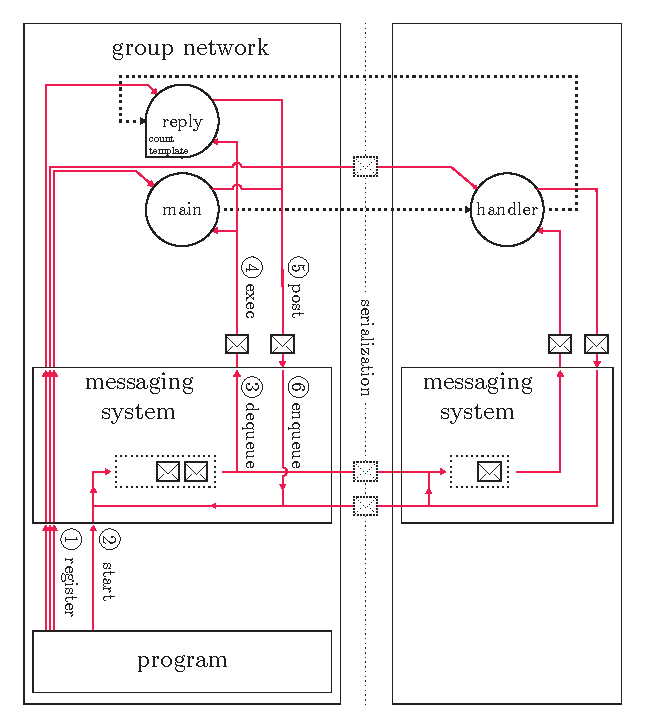
\includegraphics[width=\linewidth]{ressources/schema-message.pdf}
  \caption{Messaging system details}
  \label{fig:MesSys}
\end{figure}

The messaging system carries message streams based on the names of the recipient fluxions.
So it needs every fluxion to be registered.
If two fluxions share the same name, the messaging system would be in a conflicting situation.
This registration associates a processing function with a unique name and an initial \textit{context}.
The registration is done using the \texttt{register(<nom>, <fn>, <context>)} function, \circled{1}.
% A fluxion can dynamically register other fluxions

To trigger a chain of fluxions, a message is sent using the function \texttt{start(<msg>)}, \circled{2}.
This function pushes a first message in the queue.
Immediately, the system dequeues this message and invokes the recipient processing function, \circled{3} and \circled{4}.
The recipient function sends back messages using the function \texttt{post(<msg>)}, \circled{5}, to be enqueued in the system, \circled{6}.
The system loops through steps \circled{3} and \circled{4} until the queue is empty.
This cycle starts again for each new incoming request causing a \textit{start} message.

Algorithms \ref{alg:parcours} and \ref{alg:traitement} describe the behavior of the messaging system after the \texttt{start} function invocation.

\begin{algorithm}
\caption{Message queue walking algorithm}
\label{alg:parcours}
\begin{algorithmic}
\Function{loopMessage}{\null}
\While{$msg$ \textbf{presents in} $msgQueue$}
\State $msg \gets$ \Call{dequeue}{\null} \Comment{\circled{3}}
\State \Call{ProcessMsg}{$msg$}
\EndWhile
\EndFunction
\end{algorithmic}
\end{algorithm}

\begin{algorithm}
\caption{Message processing algorithm}
\label{alg:traitement}
\begin{algorithmic}
\Function{processMsg}{$msg$}
\For{$dest$ \textbf{in} $msg.dest$}
\State $fluxion \gets lookup(dest)$
\State $message \gets$ \Call{exec}{$fluxion, msg.body$} \Comment{\circled{4} \& \circled{5}}
\State \Call{enqueue}{$message$} \Comment{\circled{6}}
\EndFor
\EndFunction
\end{algorithmic}
\end{algorithm}

\subsection{Service example}

To illustrate the fluxional execution model, we present an example of a simple web application.
This application reads the file containing its own source code, and sends it back along with a request counter.

The original source code of this application is available on github\cite{flx-example}, and in listing \ref{lst:source}.
In this source code, some points are worth noticing.

\begin{itemize}
  \item The \texttt{reply} function, line 5 to 11, contains the logic we want to split into the fluxional processing chain.
  It receives the user request in the variable \texttt{res} which is used by the last function of the chain, \texttt{reply}.
  \item The \texttt{count} object at line 3 is a persistent memory that increments the request counter.
  This object needs to be mapped to a fluxion \textit{execution context} in the fluxional execution model.
  \item The \texttt{get} and \texttt{send} functionss, respectively line 5 and 9, interface the application with the clients.
  The processing chain of functions occurs between these two functions : $\texttt{get} \to \texttt{handler} \to \texttt{readFile} \to \texttt{reply} \to \texttt{send}$.
\end{itemize}

\includecode{js,
  caption={Simple web application. \textnormal{this application replies to every user request with its own source code and the value of a request counter}},
  label={lst:source}
}
{../../example/source.js}

This application is transformed manually into the fluxions chain depicted in Figure \ref{fig:fluxions}.
We expect a similar result with the compiler described in section \ref{section:compiler}.
Circles represent registered fluxions.
Envelope symbols represent messages streams between fluxions with the variables transmitted from one fluxion to the other.
The square in the messaging system holds the \textit{context} of the \texttt{reply} fluxion.
When a new REST request \texttt{GET} is received, a \texttt{start} message triggers the flow.
The \texttt{handler} fluxion receives this \texttt{start} message, reads the source file and forwards it to the \texttt{reply} fluxion which increments the counter, and sends the result back.
Each fluxion propagates the necessary values from one fluxion to the other exclusively by messages.
Horizontal dashed lines show virtual transmission of messages between fluxions although they all go through the messaging system.

\begin{figure}[h!]
  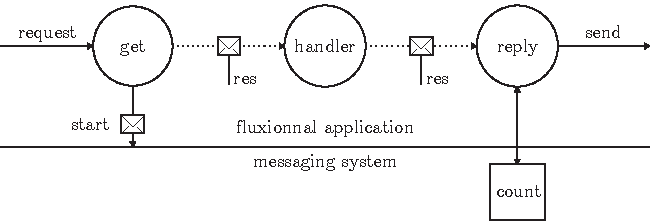
\includegraphics[width=\linewidth]{ressources/flux.pdf}
  \caption{Fluxions chain manually extracted from the example application}
  \label{fig:fluxions}
\end{figure}

Listing \ref{lst:fluxional} describes this counting application in our high-level fluxional language.
There is two types of fluxion depending on their input streams.
A fluxion with no input stream is a \textit{root} fluxion, while the others are \textit{following} fluxions.
The \textit{root} fluxion initializes the application.

There is two types of strea based on the two functions to send messages, \textit{start} and \textit{post}.
A stream is defined with an operator indicating its type, a list of recipient fluxions separated by commas, and a description of its message body. 
The operator to represent a \textit{start} stream is a double arrow, $\twoheadrightarrow$ or \texttt{>}\texttt{>}, while for a \textit{post} stream it is a single arrow, $\rightarrow$ or \texttt{->}.
The description of the message body is a comma separated list of variables identifiers enclosed in square brackets.
It is optional and only gives indications about the message content.
A stream is defined with this syntax :\\
\texttt{<operator> <recipients list> [<body description>]}\\
For the last fluxion of the chain, the output stream is a special stream called \texttt{null}.

A fluxion is defined with a header followed by a body with an indentation of two spaces.
The header starts with the keyword \texttt{flx}, followed by its name and a description of its memory \textit{cakeontext}.
After this first line, there is a list of output streams as defined above, and finally the body of the fluxion containing the processing function.
The processing function is defined with the Javascript syntax, augmented with the stream syntax to allow it to send output streams.
It can access and manipulate only two objects : \texttt{msg}, the received message and \texttt{this}, the persisted \textit{context}.
The \textit{root} fluxion is an exception, as it doesn't have input streams its body isn't a processing function but initialization code.
A fluxion is defined with this syntax :\\
\texttt{flx <name> {<context>}}\\
\texttt{<output streams>}\\
\texttt{  <processing function>}\\

% This language brings a stricter segmentation than the initial code by allowing to only register and define fluxions.
% A fluxion is defined by a name, a description of the \textit{context}, the operator \texttt{>}\texttt{>} for starting fluxions or \texttt{-}\texttt{>} for following fluxions and finally a list of downstream fluxions with the content of the message for each stream.
% The body containing the processing function is following the fluxion definition.

\begin{code}[flx, caption={Manual transformation of the example application in our high-level fluxional language},label={lst:fluxional}]
flx get
>> handler [res]
  var app = require('express')(),
      fs = require('fs'),
      count = 0;

@\label{lst:fluxional-streamtohandler}@  app.get('/', >> handler);
  app.listen(8080);
  console.log('>> listening 8080');

flx handler
-> reply [res]
  function handler(req, res) {
@\label{lst:fluxional-readfile}@      fs.readFile(__filename, -> reply);
  }

flx reply {count}
-> null
  function reply(error, data) {
@\label{lst:fluxional-counter}@    count += 1;
    var code = ('' + data).replace(/\n/g, '<br>').replace(/ /g, '&nbsp');
@\label{lst:fluxional-ressend}@    res.send('downloaded ' + count + ' times<br><br><code>' + code + '</code>');
  }
\end{code}

The application is organized as follow :
\begin{itemize}
  \item The \texttt{get} fluxion is the \textit{root} fluxion.
  It initializes the application to listen for user requests by calling \texttt{app.get}.
  Every request is forwarded on the stream to the \texttt{handler} fluxion, line \ref{lst:fluxional-streamtohandler}.
  \item The \texttt{handler} fluxion reads the file containing the source code of the application, and forwards the result to the \texttt{reply} fluxion, line \ref{lst:fluxional-readfile}.
  \item The \texttt{reply} fluxion increments the counter, line \ref{lst:fluxional-counter}, formats the reply, and sends it back to the user using the function \texttt{res.send}, line \ref{lst:fluxional-ressend}.
\end{itemize}

Our goal, as described in the introduction, is not to propose a new programming paradigm with this high-level language but to automate the architecture shift with a compiler.